\clearpage
\setcounter{page}{1}
\maketitlesupplementary
\setcounter{section}{0}
\renewcommand{\thesection}{\Alph{section}}
% Float placement for the supplement: allow several floats per page and fuller float pages.
\setcounter{topnumber}{4}\setcounter{dbltopnumber}{4}\setcounter{totalnumber}{8}
\renewcommand{\topfraction}{0.95}\renewcommand{\dbltopfraction}{0.95}\renewcommand{\textfraction}{0.05}
\renewcommand{\floatpagefraction}{0.05}\renewcommand{\dblfloatpagefraction}{0.3}

\noindent This supplement contains the ablation study (\cref{sec:supp_ablation}), the evaluation on SD Inpainting (\cref{sec:supp_inpainting}), the settings of the baselines and the evaluation protocol (\cref{sec:supp_protocol}), and the details of the ISR evaluation (\cref{sec:supp_isr}).

\section{Ablation Study}
\label{sec:supp_ablation}
We evaluate the contributions of the components of \capg{} and compare its parameterization with simpler color mappings. \Cref{tab:ablation} reports the results, and \cref{fig:ablation_appearance} illustrates the immunized images of one portrait. All optimized variants share the solver of \capg{}: Adam for 1800 steps with the learning rate decayed from $3\times10^{-4}$ to $10^{-5}$, initial parameters drawn as $0.002\cdot\mathcal{N}(0, 1)$ around the identity mapping, and the objective of \capg{}, the distance between the posterior means of the InstructPix2Pix VAE encoder for the immunized and the original image. No distortion constraint enters the optimization, and all outputs are clipped to $[0, 1]$.

\paragraph{Component Variants.} Each variant changes one component of \capg{} and keeps the others.
(A1)~\emph{Without optimization}: $\Theta$ is replaced by a sample $Z \sim \mathcal{N}(0, 1)$ of the same shape ($33^3 \times 3$), drawn with a seed per portrait, and passes through the same Gaussian smoothing ($\sigma = 4$) and angular bounds ($\theta_{\max} = 25^\circ$, $\phi_{\max} = 7.5^\circ$); the norm $\|c\|$ is kept and the magnitude of $Z$ is not rescaled.
(A2)~\emph{Without smoothing}: $\sigma = 0$, so that the rotation of each lattice node is optimized independently; the angular bounds and the solver are those of \capg{}.
(A3)~\emph{Without angular bounds}: the polar and azimuthal components are not passed through the saturating function $s(\cdot)$. The rotated color is still normalized to $\|c\|$, so the rotation is limited only by the orthogonality of the tangent vector to $c$, that is, to less than $90^\circ$.
(A4)~\emph{Single angular bound}: the separate bounds on $\theta$ and $\phi$ are replaced by one bound on the total rotation. The tangent vector $V_\perp$ is saturated as $\tan 25^\circ \cdot \tanh(\|V_\perp\| / \tan 25^\circ)$, so that the chromatic direction measured from black rotates by less than $25^\circ$ in any direction; $\sigma = 4$ and $\|c\|$ are kept.

\paragraph{Alternative Color Mappings.} The parameterization of \capg{} is a design of this work; we therefore compare it with simpler and more direct parameterizations of a color mapping. Each mapping is matched to the defense LPIPS of \capg{} on the same portrait.
B1 and B2 use a two-parameter model, a global rotation about the gray axis combined with a scaling of the distance to it: $c' = m + e^{s} R_u(h)\,(c - m)$, where $m$ is the projection of $c$ onto the gray axis, $R_u(h)$ is the rotation by $h$ about $u = (1, 1, 1)/\sqrt{3}$ in RGB, and $e^{s}$ scales the distance to the gray axis.
(B1)~\emph{Random rotation and scaling}: $(h, s) = \alpha\,(z_h, z_s)$ with $(z_h, z_s) \sim \mathcal{N}(0, 1)^2$ drawn with a seed per portrait, and $\alpha$ is found by bisection on a logarithmic scale so that the defense LPIPS lies within $\pm 0.005$ of that of \capg{}. With $|h|$ capped at $\pi$, the target distortion is not reachable on 34 portraits, for which the mapping at the cap is used.
(B2)~\emph{Optimized rotation and scaling}: the two scalars $(h, s)$ are optimized with the solver of \capg{}.
(B3)~\emph{Optimized $3\times3$ affine}: $c' = A c + b$ in RGB with 12 parameters, optimized from the identity.
(B4)~\emph{Unconstrained $K^3$ LUT}: the $33^3 \times 3$ vertex displacements of a LUT are optimized without smoothing or angular bounds.
For B2 to B4, only checkpoints whose defense LPIPS, measured on the quantized image, lies within $\pm 0.015$ of that of \capg{} on the same portrait are kept.

\paragraph{Effect of Optimization and Geometric Constraints.} Without optimization (A1), a random $\Theta$ changes the image only slightly: the defense LPIPS is 0.045 and the edit LPIPS without purification is 0.087, compared with 0.287 and 0.353 for \capg{}, while LAION and MUSIQ are higher by 0.12 and 0.06. Removing the Gaussian smoothing (A2), removing the angular bounds (A3), or replacing the separate bounds on $\theta$ and $\phi$ with a single rotation bound (A4) increases the defense LPIPS by 0.114 to 0.172 and the edit LPIPS by 0.109 to 0.154 without purification and by 0.034 to 0.140 after VAE-Trans. These variants also reduce MUSIQ by 0.14 to 0.34; LAION decreases by 0.04 and 0.08 for A2 and A3, and is 5.33 for A4, compared with 5.32 for \capg{}. In \cref{fig:ablation_appearance}, A2 shows irregular color patches in the background and on the face, and A3 and A4 shift the colors of the background, the face, and the hair.

\paragraph{Comparison with Alternative Color Mappings.} At matched defense LPIPS (differences from \capg{} of at most 0.004), the optimized rotation and scaling (B2) yields edit LPIPS within 0.007 of \capg{} without purification and after JPEG~50 and blur~2, and 0.029 higher after VAE-Trans. The optimized affine transformation (B3) yields edit LPIPS higher by 0.029 to 0.076, and the unconstrained LUT (B4) yields edit LPIPS higher by 0.027 without purification and by 0.017 after VAE-Trans but lower by 0.011 after JPEG~50 and by 0.041 after blur~2. All three mappings have lower MUSIQ than \capg{}, by 0.17 (B2), 0.50 (B3), and 0.25 (B4), and lower LAION, by 0.13, 0.06, and 0.02. The random rotation and scaling (B1) does not reach the target distortion on every portrait (defense LPIPS 0.238); its edit LPIPS is lower than that of \capg{} by 0.033 to 0.055, and its MUSIQ and LAION are lower by 0.11 and 0.04. In \cref{fig:ablation_appearance}, B2 desaturates the whole image, B3 adds a pale pink cast, and B4 changes the hue of individual colors, such as the red checks of the shirt.

\begin{figure*}[t]
  \centering
  % Each source PDF holds five 100.32 bp panels; the viewports cut out the panels used here.
  \makebox[0.185\textwidth]{}\makebox[0.185\textwidth]{\small A2}\makebox[0.185\textwidth]{\small A3}\makebox[0.185\textwidth]{\small A4}\\[1pt]
  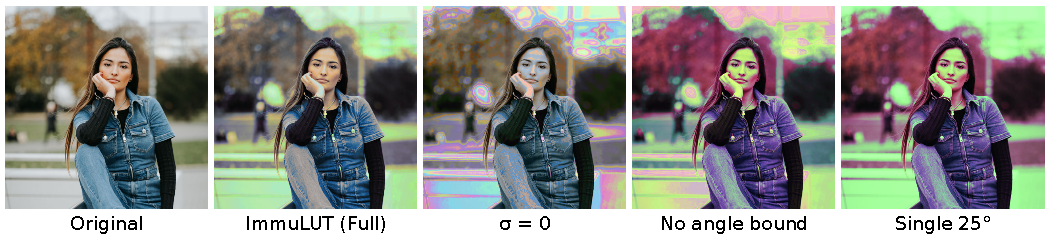
\includegraphics[viewport=1.2 0 101.52 116.64, clip, width=0.185\textwidth]{fig/ablation_components.pdf}%
  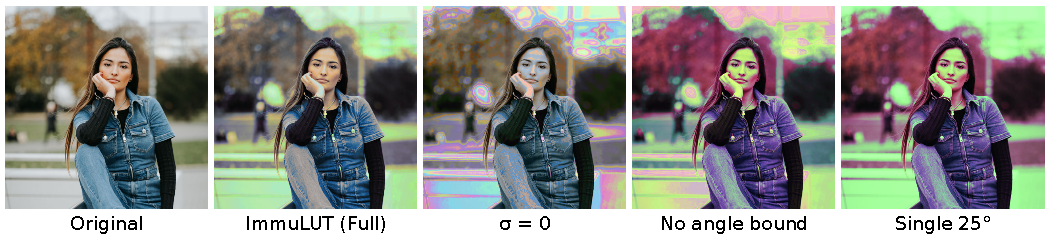
\includegraphics[viewport=201.84 0 502.80 116.64, clip, width=0.555\textwidth]{fig/ablation_components.pdf}\\[2pt]
  \makebox[0.185\textwidth]{\small Full}\makebox[0.185\textwidth]{\small B2}\makebox[0.185\textwidth]{\small B3}\makebox[0.185\textwidth]{\small B4}\\[1pt]
  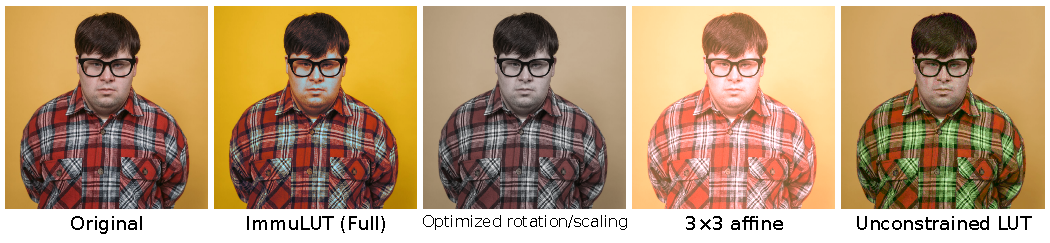
\includegraphics[viewport=101.52 0 201.84 116.64, clip, width=0.185\textwidth]{fig/ablation_appearance.pdf}%
  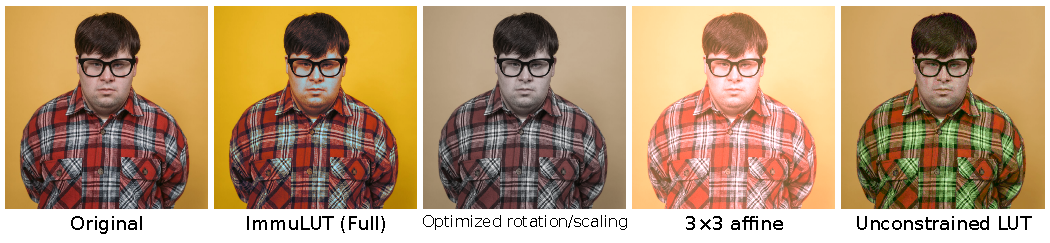
\includegraphics[viewport=201.84 0 502.80 116.64, clip, width=0.555\textwidth]{fig/ablation_appearance.pdf}
  \caption{Immunized images of one portrait under the variants of \cref{tab:ablation}. Left: the original (top) and \capg{} (bottom). Labels above the panels give the variant codes of \cref{tab:ablation}. Top row: the variants that change one component, at different defense LPIPS. Bottom row: the simpler color mappings, each optimized to the defense LPIPS of \capg{} on this portrait (0.127) within $\pm 0.015$.}
  \label{fig:ablation_appearance}
\end{figure*}

\begin{table*}[t]
  \centering
  \footnotesize
  \setlength{\tabcolsep}{4pt}
  \caption{Ablations on InstructPix2Pix (306 portraits $\times$ 4 instructions). B1 does not reach the target distortion on 34 portraits. For four portraits, the solver runs for 3600 steps with a fixed learning rate: B2 on woman\_44 ($3\times10^{-4}$), woman\_82, and woman\_129, and B3 on man\_99 ($10^{-3}$). Best in bold.}
  \label{tab:ablation}
  \begin{tabular}{@{}ll ccc cccc@{}}
    \toprule
    & & \multicolumn{3}{c}{Immunized image} & \multicolumn{4}{c}{Edit LPIPS $\uparrow$} \\
    \cmidrule(lr){3-5} \cmidrule(l){6-9}
    & Variant & LPIPS $\downarrow$ & LAION $\uparrow$ & MUSIQ $\uparrow$ & None & JPEG 50 & Blur 2 & VAE-Trans \\
    \midrule
    \rowcolor{oursrow}
    Full & \capg{} (Ours) & .287 & 5.32 & 5.30 & .353 & .386 & .360 & .288 \\
    \midrule
    \multicolumn{9}{@{}l}{\emph{Components (unmatched distortion)}} \\
    A1 & w/o optimization (random $\Theta$) & \textbf{.045} & \textbf{5.44} & \textbf{5.36} & .087 & .151 & .082 & .061 \\
    A2 & w/o smoothing ($\sigma = 0$) & .401 & 5.28 & 5.05 & .462 & .448 & .425 & .322 \\
    A3 & w/o angle bounds & .459 & 5.24 & 4.96 & \textbf{.507} & \textbf{.530} & \textbf{.517} & .421 \\
    A4 & single angle bound ($25^\circ$) & .437 & 5.33 & 5.16 & .483 & .518 & .505 & \textbf{.428} \\
    \midrule
    \multicolumn{9}{@{}l}{\emph{Color mappings (matched distortion)}} \\
    B1 & random rotation / scaling & .238 & 5.28 & 5.19 & .298 & .337 & .317 & .255 \\
    B2 & optimized rotation / scaling & .291 & 5.19 & 5.13 & .355 & .393 & .366 & .317 \\
    B3 & optimized $3\times3$ affine & .288 & 5.26 & 4.80 & .382 & .428 & .394 & .364 \\
    B4 & unconstrained $K^3$ LUT & .289 & 5.30 & 5.05 & .380 & .375 & .319 & .305 \\
    \bottomrule
  \end{tabular}
\end{table*}

\section{Cross-Editor Evaluation on SD Inpainting}
\label{sec:supp_inpainting}
We further evaluate the transferability of the immunization to a mask-based inpainting editor, in which the edit is confined to a region outside the person.

\paragraph{Experimental Setup.} We use Stable Diffusion Inpainting (\texttt{runwayml/stable-diffusion-inpainting}, based on SD~1.5). Its VAE is identical to that of InstructPix2Pix, and we apply the immunized images optimized against InstructPix2Pix without re-optimization. The mask is the complement of a subject mask produced with CLIPSeg (\texttt{CIDAS/clipseg-rd64-refined}, the class name as text prompt, threshold 0.30, dilation by 4 pixels), so that only the background is repainted, and the output is composited with the input outside the mask. We use 50 sampling steps, a guidance scale of 7.5, strength 1.0, and seed 20260812 at $512\times512$. Following DiffusionGuard~\cite{diffusionguard2025}, we adopt four inpainting prompts: ``A man/woman in a hospital'', ``\ldots{} in the gym'', ``\ldots{} in a snowy street'', and ``\ldots{} sitting next to a dog''. We compare \capg{} with PhotoGuard, DIA-PT, DCT-Shield, SIFM, and BlurGuard in their matched-distortion settings, without purification and after JPEG~50, Gaussian blur ($\sigma = 2$), and VAE-Trans, resulting in 1{,}224 edits per method and purification on the 306 portraits. In \cref{tab:supp_inpainting,tab:supp_inpaint_isr}, the additive defenses use the matched-distortion settings of \cref{tab:main}, with the same budget scaling factors as for InstructPix2Pix; in \cref{fig:supp_inpaint_man_26,fig:supp_inpaint_woman_14,fig:supp_inpaint_dog,fig:supp_inpaint_snowy}, they use their native budgets, and BlurGuard uses its official setting ($\epsilon = 16/255$, 150 steps). As in \cref{tab:main}, each metric compares the edit of the immunized image with the edit of the original image under the same purification.

\paragraph{Quantitative and Qualitative Comparison.} As shown in \cref{tab:supp_inpainting}, without purification, the additive defenses yield edit LPIPS between 0.270 and 0.322, and \capg{} yields 0.378. After purification, the edit LPIPS of the additive defenses decreases to between 0.044 and 0.234, with BlurGuard retaining the highest values, whereas that of \capg{} remains between 0.352 and 0.389. SigLIP and ArcFace similarities follow the same trend: after blur, \capg{} yields 0.862 and 0.906, compared with at least 0.951 and 0.954 for the additive defenses. \Cref{fig:supp_inpaint_man_26,fig:supp_inpaint_woman_14} show two portraits with the additive defenses at their native budgets. After purification, the requested content appears in the edits of the undefended image and of PhotoGuard, DIA-PT, DCT-Shield, and SIFM, and only partially in the edit of BlurGuard, whereas the edits of \capg{} keep the original background with and without purification. \Cref{fig:supp_inpaint_dog,fig:supp_inpaint_snowy} show two further portraits, with the dog and snowy street prompts. After purification, the edits of the undefended image and of at least four of the five additive defenses carry out the prompt, while the edit of \capg{} does not.

\paragraph{Immunization Success Rate.} We also measure the ISR of the inpainting edits on the 306 portraits and four prompts. For each portrait and prompt, one sheet shows the input and the four edits (without purification, after JPEG~50, after blur, and after VAE-Trans) of the original image and of the six immunized images; the seven rows are shuffled independently for each sheet and are labeled without method names, giving 1{,}224 sheets. Claude Sonnet~5.5 assigns three binary labels to every edit: \emph{content}, whether the requested background content is clearly present; \emph{mismatch}, whether the edit alters the person, adds people, or produces content other than the request; and \emph{degraded}, whether the image shows a severe structural or quality breakdown. A global color cast alone is not counted as a failure. An edit succeeds when the content is present and neither mismatch nor degradation occurs. The ISR is conditional: it counts only the portrait--prompt pairs on which the edit of the original image succeeds under the same purification, and an immunized edit counts as an immunization success when any of the three labels fails. The edits of the original image succeed in 68.7\%, 72.3\%, 65.8\%, and 66.5\% of the 1{,}224 pairs without purification and after JPEG~50, blur, and VAE-Trans, respectively. Intervals are 95\% bootstrap intervals over portraits with 1{,}000 resamples. Two differences from the protocol of \cref{tab:isr} apply: the inpainting judgments are not reviewed by hand, and the color shift of the images immunized by \capg{} is visible in the sheets, so the blinding is incomplete for this row. As shown in \cref{tab:supp_inpaint_isr}, without purification, the additive defenses yield ISR between 10.5\% and 13.4\%, and \capg{} yields 23.7\%. After purification, the ISR of the additive defenses is between 2.4\% and 9.4\%, and that of \capg{} is between 23.1\% and 28.7\%; over the three purifications combined, \capg{} yields 25.8\% and BlurGuard 8.3\%.

\begin{table*}[t]
  \centering
  \footnotesize
  \setlength{\tabcolsep}{5pt}
  \caption{Immunization Success Rate on SD Inpainting (306 portraits $\times$ 4 prompts, Claude Sonnet~5.5 without human review). Combined: the three purifications pooled. Brackets: 95\% bootstrap interval over portraits.}
  \label{tab:supp_inpaint_isr}
  \begin{tabular}{@{}lccccc@{}}
    \toprule
    & & \multicolumn{4}{c}{Purified} \\
    \cmidrule(l){3-6}
    Method & None & JPEG 50 & Blur 2 & VAE-Trans & Combined \\
    \midrule
    PhotoGuard & 13.4 {\scriptsize[10.9, 16.1]} & 4.4 {\scriptsize[3.2, 5.8]} & 3.7 {\scriptsize[2.4, 5.2]} & 5.3 {\scriptsize[3.7, 7.1]} & 4.5 {\scriptsize[3.6, 5.4]} \\
    DIA-PT & 11.1 {\scriptsize[8.8, 13.3]} & 5.4 {\scriptsize[4.0, 6.9]} & 4.6 {\scriptsize[3.2, 6.1]} & 4.7 {\scriptsize[3.3, 6.2]} & 4.9 {\scriptsize[4.1, 5.8]} \\
    DCT-Shield & 10.5 {\scriptsize[8.5, 12.6]} & 2.4 {\scriptsize[1.4, 3.4]} & 2.6 {\scriptsize[1.5, 3.7]} & 5.2 {\scriptsize[3.7, 6.8]} & 3.4 {\scriptsize[2.7, 4.2]} \\
    SIFM & 13.2 {\scriptsize[11.1, 15.6]} & 4.5 {\scriptsize[3.2, 5.8]} & 4.7 {\scriptsize[3.2, 6.4]} & 3.8 {\scriptsize[2.6, 5.1]} & 4.4 {\scriptsize[3.5, 5.2]} \\
    BlurGuard & 12.7 {\scriptsize[10.4, 15.1]} & 9.4 {\scriptsize[7.5, 11.4]} & 8.0 {\scriptsize[6.1, 9.9]} & 7.6 {\scriptsize[5.6, 9.7]} & 8.3 {\scriptsize[7.0, 9.8]} \\
    \midrule
    \rowcolor{oursrow}
    \textbf{\capg{} (Ours)} & \textbf{23.7} {\scriptsize[20.6, 27.2]} & \textbf{23.1} {\scriptsize[20.1, 26.1]} & \textbf{28.7} {\scriptsize[25.5, 32.2]} & \textbf{25.9} {\scriptsize[22.8, 29.4]} & \textbf{25.8} {\scriptsize[23.5, 28.5]} \\
    \bottomrule
  \end{tabular}
\end{table*}

\begin{table*}[t]
  \centering
  \footnotesize
  \setlength{\tabcolsep}{3.5pt}
  \caption{SD Inpainting (306 portraits $\times$ 4 instructions; immunized images optimized against InstructPix2Pix, without re-optimization). Each metric compares the edit of the immunized image with the edit of the original under the same purification. Best means in bold. ArcFace finds no face in the edits of one portrait after blur and after VAE-Trans; these cells are excluded from the ArcFace means.}
  \label{tab:supp_inpainting}
  \begin{tabular}{@{}l c cccc cccc cccc@{}}
    \toprule
    & Immunized & \multicolumn{4}{c}{Edit LPIPS $\uparrow$} & \multicolumn{4}{c}{SigLIP $\downarrow$} & \multicolumn{4}{c}{ArcFace $\downarrow$} \\
    \cmidrule(lr){3-6} \cmidrule(lr){7-10} \cmidrule(l){11-14}
    Method & LPIPS $\downarrow$ & None & JPEG 50 & Blur 2 & VAE & None & JPEG 50 & Blur 2 & VAE & None & JPEG 50 & Blur 2 & VAE \\
    \midrule
    PhotoGuard & .318 & .322 & .134 & .053 & .072 & .950 & .978 & .984 & .985 & .983 & .970 & .989 & .984 \\
    DIA-PT & .261 & .280 & .160 & .075 & .086 & .952 & .970 & .977 & .983 & .976 & .966 & .979 & .972 \\
    DCT-Shield & .283 & .283 & .109 & .044 & .061 & .958 & .980 & .986 & .987 & .987 & .980 & .989 & .987 \\
    SIFM & \textbf{.251} & .270 & .150 & .071 & .082 & .952 & .973 & .978 & .983 & .978 & .969 & .984 & .979 \\
    BlurGuard & .275 & .283 & .234 & .171 & .156 & .944 & .948 & .951 & .968 & .961 & .946 & .954 & .955 \\
    \midrule
    \rowcolor{oursrow}
    \textbf{\capg{} (Ours)} & .287 & \textbf{.378} & \textbf{.389} & \textbf{.386} & \textbf{.352} & \textbf{.887} & \textbf{.888} & \textbf{.862} & \textbf{.897} & \textbf{.944} & \textbf{.924} & \textbf{.906} & \textbf{.895} \\
    \bottomrule
  \end{tabular}
\end{table*}

\begin{figure*}[t]
  \centering
  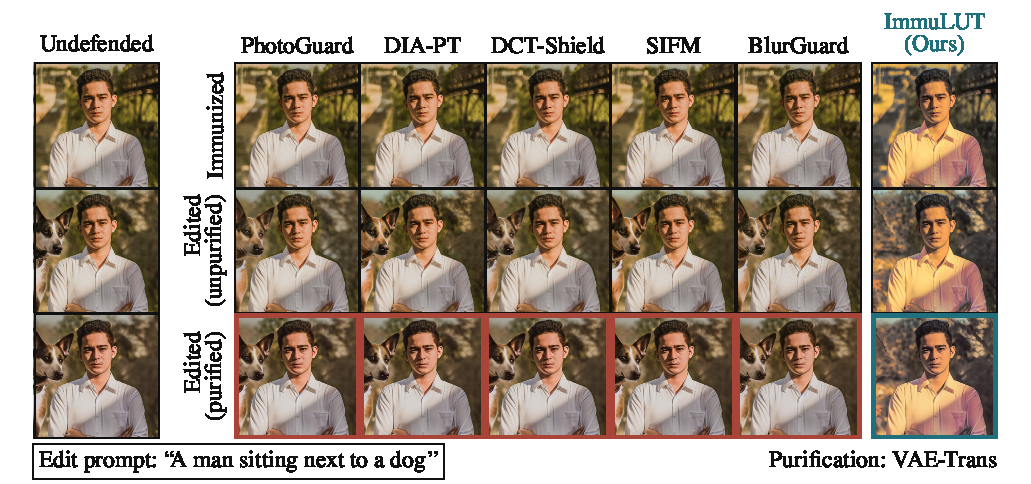
\includegraphics[width=0.85\textwidth]{fig/inpaint_man_26_dog.pdf}
  \caption{Edits with the prompt ``A man sitting next to a dog'' on SD Inpainting, with the additive defenses at their native budgets. Rows: immunized image, edit without purification, and edit after VAE-Trans. After VAE-Trans, the edits of the undefended image and of PhotoGuard, DIA-PT, DCT-Shield, and SIFM add a dog, the edit of BlurGuard shows part of a dog head at the left border, and the edit of \capg{} shows no dog. Edit LPIPS after VAE-Trans: PhotoGuard .062, DIA-PT .046, DCT-Shield .039, SIFM .095, BlurGuard .217, and \capg{} .394.}
  \label{fig:supp_inpaint_man_26}
\end{figure*}

\begin{figure*}[t]
  \centering
  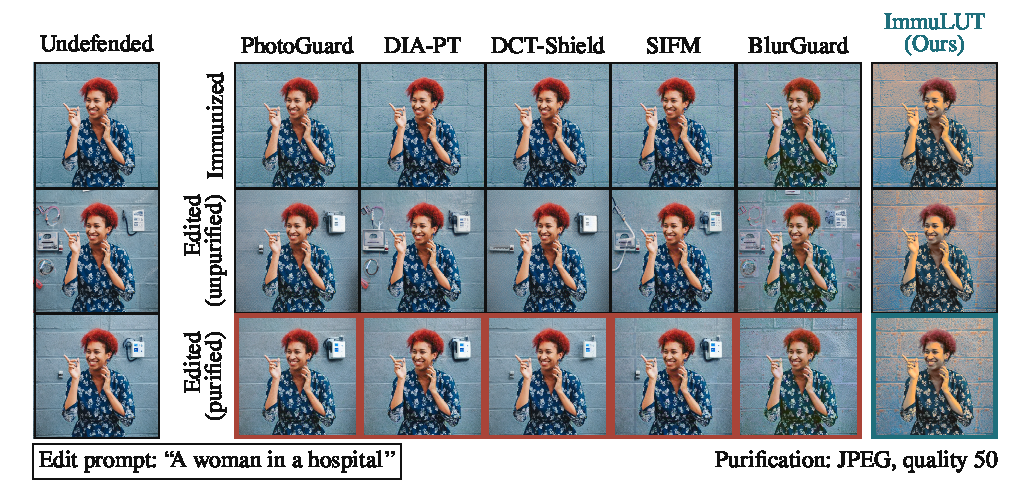
\includegraphics[width=0.85\textwidth]{fig/inpaint_woman_14_hospital.pdf}
  \caption{Edits with the prompt ``A woman in a hospital'' on SD Inpainting, with the additive defenses at their native budgets. Rows: immunized image, edit without purification, and edit after JPEG compression (quality 50). After compression, the edits of the undefended image and of PhotoGuard, DIA-PT, DCT-Shield, and SIFM add wall-mounted medical equipment, the edit of BlurGuard adds a few small objects to the wall, and the edit of \capg{} keeps the brick wall. Edit LPIPS after JPEG compression: PhotoGuard .168, DIA-PT .165, DCT-Shield .080, SIFM .234, BlurGuard .273, and \capg{} .399.}
  \label{fig:supp_inpaint_woman_14}
\end{figure*}

\begin{figure*}[t]
  \centering
  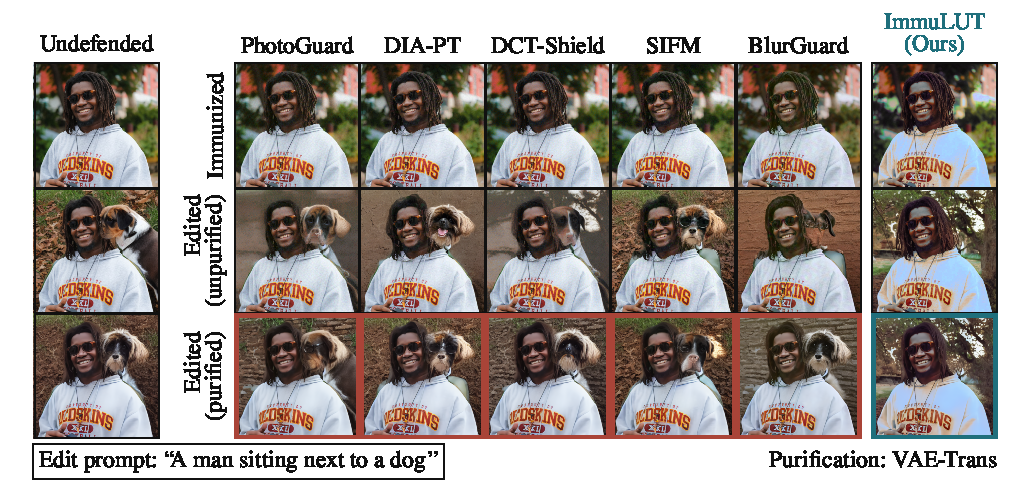
\includegraphics[width=0.85\textwidth]{fig/inpaint_man_81_dog.pdf}
  \caption{Edits with the prompt ``A man sitting next to a dog'' on SD Inpainting, with the additive defenses at their native budgets. Rows: immunized image, edit without purification, and edit after VAE-Trans. After VAE-Trans, the edits of the undefended image and of the five additive defenses add a dog beside the person, and the edit of \capg{} shows no dog. Edit LPIPS after VAE-Trans: PhotoGuard .271, DIA-PT .128, DCT-Shield .186, SIFM .189, BlurGuard .267, and \capg{} .389.}
  \label{fig:supp_inpaint_dog}
\end{figure*}

\begin{figure*}[t]
  \centering
  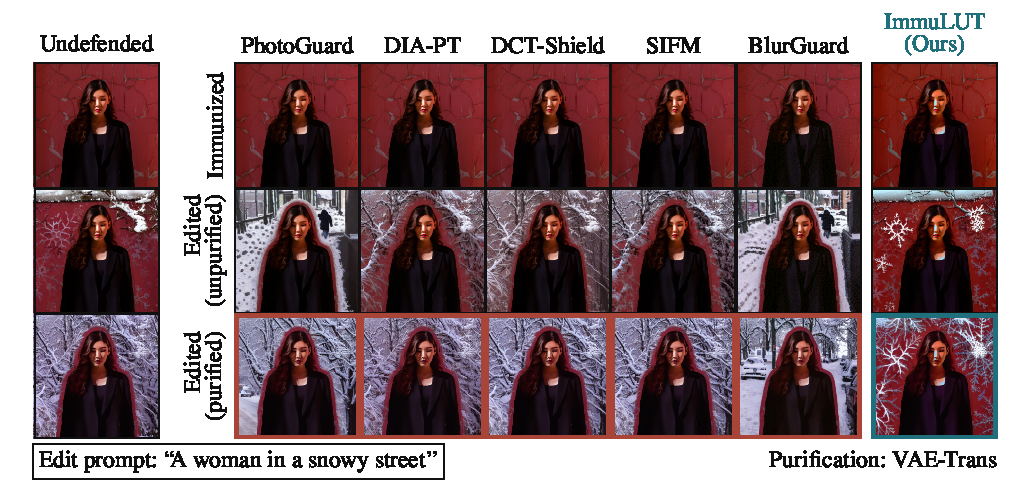
\includegraphics[width=0.85\textwidth]{fig/inpaint_woman_118_snowy_street.pdf}
  \caption{Edits with the prompt ``A woman in a snowy street'' on SD Inpainting, with the additive defenses at their native budgets. Rows: immunized image, edit without purification, and edit after VAE-Trans. After VAE-Trans, the edits of the undefended image and of the five additive defenses show a snowy street, whereas the edit of \capg{} keeps the red background with white snowflake-like patterns and shows no street. Edit LPIPS after VAE-Trans: PhotoGuard .380, DIA-PT .132, DCT-Shield .277, SIFM .268, BlurGuard .405, and \capg{} .395.}
  \label{fig:supp_inpaint_snowy}
\end{figure*}


\section{Baseline and Protocol Details}
\label{sec:supp_protocol}
\paragraph{Data.} We select the portraits from the metadata of a public collection of 9{,}853 Pexels portraits in which every image contains a detected face, and download each image at a width of 1200 pixels. The selection consists of six steps. (1)~We keep images whose description contains words for exactly one of man and woman and none of a list of exclusion words (children, groups, black-and-white, occlusion, artistic rendering), which leaves 5{,}763 images. (2)~We require that MTCNN detects exactly one face with probability at least 0.98, that the face height is 0.07 to 0.50 of the shorter image side, that the face is near-frontal (horizontal offset of the nose tip at most 0.25 of the inter-eye distance), that the image is not grayscale (mean $|a^*| + |b^*| \ge 6$ in CIELAB), and that the face box lies inside the crop, which leaves 2{,}486 images. (3)~We require that the zero-shot gender probability of CLIP ViT-L/14 is at least 0.8 and agrees with the description, and that FaceNet returns an identity embedding, which leaves 2{,}459 images (407 men and 2{,}052 women). (4)~We rank the images by CLIP image similarity to eight reference portraits, keep at most two images per photographer, and treat pairs with FaceNet identity cosine similarity of at least 0.65 as the same person. (5)~We remove images with occlusion, profile views, closed eyes, small subjects, face paint, children, nudity, or underexposure by visual inspection. (6)~We remove six images whose subject mask covers less than 1\% or more than 80\% of the image or misses the person. The gender ratio of the resulting set follows the number of men that pass step~(3). We record the Pexels identifier, photographer, description, original size, face box, crop box, and checksum of each image. We crop each portrait to a square of side $\min(H, W)$ centered $0.18$ side lengths below the center of the detected face box, clamp the square to the image, and resize it to $512\times512$ with Lanczos resampling. We obtain subject masks with CLIPSeg (\texttt{CIDAS/clipseg-rd64-refined}, the class name as text prompt, threshold 0.30, dilation by 4 pixels); the masks define the inpainting region in \cref{sec:supp_inpainting} and are not used by any defense.

\paragraph{Purifications.} Cropping removes 10\% from each side and resizes the result to $512\times512$ with bicubic interpolation; rotation uses bilinear interpolation and zero fill. Each purification is applied to the immunized image, and the edit of the purified image is compared with the edit of the original image under the same purification. VAE-Trans reconstructs the immunized image through a VAE whose encoder is fine-tuned on clean images.

\paragraph{VAE-Trans.} We reproduce VAE-Trans~\cite{purifyonce2026} on the VAE of InstructPix2Pix (\texttt{timbrooks/instruct-pix2pix}, revision 31519b5). Only the encoder and the quantization convolution are fine-tuned; the decoder is frozen. The input is $x + \eta$ with $\eta \sim \mathcal{N}(0, 0.1^2)$ on the $[0, 1]$ scale, and the target is the posterior mean of the frozen original encoder for the clean image $x$, with a mean squared error loss. Following the paper, we use AdamW with learning rate $10^{-4}$ for 6 epochs; the batch size of 2 and random $512\times512$ crops are our choices, as the paper does not state them. Training uses 2{,}000 OmniEdit images, validation 64, and seed 0; the validation latent error decreases from 16.99 to 3.33. At inference, the purified image is the decoding of the posterior mean of the fine-tuned encoder, without sampling, at $512\times512$.

\paragraph{Editors.} For cross-model transferability, we use VIBE-DistilledCFG (\texttt{iitolstykh/VIBE-Image-Edit-DistilledCFG}, revision a10edb9, 20 sampling steps, other settings at the pipeline defaults) and the distilled FLUX.2 [klein] 4B (\texttt{black-forest-labs/FLUX.2-klein-4B}, revision e7b7dc2, bf16, 4 steps, guidance 1.0) at $512\times512$ with seed 20260812; both receive the instructions in the form ``Add sunglasses to the person''. The undefended edit of each image and instruction uses the same seed as the immunized edit, so that the two differ only in the input image. All editors receive the immunized images obtained against InstructPix2Pix, without re-optimization. The inpainting editor (\texttt{runwayml/stable-diffusion-inpainting}, revision 8a4288a, fp32) is described in \cref{sec:supp_inpainting}.

\paragraph{Matched-Distortion Rescaling.} We first run each additive defense at the budget of its paper (\cref{tab:supp_provenance}). To approximately match perceptual distortion, we multiply the budget $\epsilon$ by a factor chosen on a calibration set of 8 portraits so that the mean defense LPIPS equals 0.3344, the value of an earlier color-based variant, and apply the factors unchanged to the 306 portraits. We scale the step size by the same factor so that the ratio of step size to budget is unchanged, and keep all other settings. The rescaled settings therefore differ from those of the original papers; for DCT-Shield and DCT-Shield-Y, the rescaled budget falls below one quantization level, so the condition under which these papers state robustness to JPEG compression no longer holds. LPIPS is computed with \texttt{piq.LPIPS} (VGG) on the delivered 8-bit images.

\paragraph{Baseline Settings.} \Cref{tab:supp_provenance} lists the native settings of each additive defense, the factor applied to its budget in the matched-distortion setting, and the source of the implementation. We port the official code where it is available and otherwise reimplement the method from the description in its paper.

\begin{table*}[t]
  \centering
  \footnotesize
  \setlength{\tabcolsep}{5pt}
  \caption{Native settings of the additive methods, the factor applied to $\epsilon$ in the matched-distortion arm, and the source of the implementation. Budgets are on the $[0, 1]$ pixel scale unless stated. Official: the authors' code, ported to this pipeline (commit in parentheses); Reimpl.: reimplemented from the paper. $^{a}$The code path enabled in the official notebook; the paper (Table~9) states an $L_\infty$ budget of 16/255 with step 2/255. $^{b}$Budget on the DCT coefficients with sign updates, step size $\eta_i = (1 - i/N)\,\gamma$ at step $i$ of $N$ with $\gamma = 0.1$, $Q_{\mathrm{alg}} = 0.95$ (0.85 for DCT-Shield-Y, luminance only); reimplemented from Algorithm~1 of the paper's supplement; in the matched-distortion arm, $\gamma$ is scaled by the same factor as $\epsilon$. $^{c}$Learning rate; $\sigma$-weighting 10. In the matched-distortion arm the $\sigma$-weighting is 0 and the solved perturbation is multiplied by 0.6071. $^{d}$Official code; the commit is not recorded. $^{e}$The paper states $\epsilon = 0.06$ and the step $2/255$ on the $[-1, 1]$ scale.}
  \label{tab:supp_provenance}
  \begin{tabular}{@{}l l l c l c l@{}}
    \toprule
    Method & Budget $\epsilon$ & Step size & Steps & Norm & $\epsilon$ factor & Source \\
    \midrule
    PhotoGuard (encoder)~\cite{salman2023photoguard} & 0.03$^{a}$ & 0.01$^{a}$ & 1000 & $L_\infty$, sign PGD & 0.2614 & Official (686bea7) \\
    Mist~\cite{liang2023mist} & 16/255 & 1/255 & 100 & $L_\infty$ & 0.125 & Official (99f5f3c) \\
    DIA-PT~\cite{dia2025} & 6.4/255 & 1/255 & 20 & $L_\infty$ & 0.418 & Official$^{d}$ \\
    DIA-R~\cite{dia2025} & 6.4/255 & 1/255 & 20 & $L_\infty$ & 0.969 & Official$^{d}$ \\
    DCT-Shield~\cite{dctshield2025} & 1$^{b}$ & $\gamma$, linearly decayed$^{b}$ & 1000 & DCT, sign$^{b}$ & 0.211 & Reimpl. \\
    DCT-Shield-Y~\cite{dctshield2025} & 1$^{b}$ & $\gamma$, linearly decayed$^{b}$ & 1000 & DCT, Y only, sign$^{b}$ & 0.073 & Reimpl. \\
    SIFM~\cite{dong2025sifm} & 7.65/255 & 1/255 (not stated) & 100 & $L_\infty$ & 0.289 & Reimpl. \\
    DAYN~\cite{lo2024dayn} & 0.03$^{e}$ & 1/255 (not stated)$^{e}$ & 100 & $L_\infty$ & 0.43 & Reimpl. \\
    DANP~\cite{zhang2025danp} & 0.03 & 1/255 (not stated) & 100 & $L_\infty$ & 0.323 & Reimpl. \\
    BlurGuard~\cite{blurguard2025} & 16/255 & 0.06$^{c}$ & 150 & $L_\infty$ & 0.6071$^{c}$ & Official (e1b2d5e) \\
    \bottomrule
  \end{tabular}
\end{table*}

\begin{table*}[t]
  \centering
  \footnotesize
  \setlength{\tabcolsep}{4pt}
  \caption{Immunization success rate (\%) on 306 portraits $\times$ 4 instructions, InstructPix2Pix, with the 95\% bootstrap interval over images. Combined: the three purifications pooled. $n$: cells whose undefended edit succeeds.}
  \label{tab:supp_isr_full}
  \begin{tabular}{@{}l ccccc@{}}
    \toprule
    Method & None & JPEG 50 & Blur 2 & VAE-Trans & Combined \\
    \midrule
    PhotoGuard & \textbf{43.6} [39.6, 47.7] & 3.3 [2.1, 4.6] & 3.4 [2.2, 4.6] & 2.8 [1.7, 4.0] & 3.2 [2.5, 3.9] \\
    DCT-Shield & 24.0 [21.1, 27.0] & 2.2 [1.3, 3.1] & 2.9 [1.8, 4.0] & 2.9 [1.9, 4.1] & 2.6 [2.0, 3.3] \\
    BlurGuard & 13.3 [11.3, 15.3] & 11.0 [9.0, 13.1] & 9.0 [7.2, 10.7] & 6.7 [5.1, 8.4] & 8.9 [7.7, 10.3] \\
    SIFM & 15.8 [13.2, 18.4] & 5.7 [4.2, 7.4] & 5.0 [3.7, 6.6] & 5.5 [4.1, 7.0] & 5.4 [4.4, 6.5] \\
    Mist & 30.9 [28.2, 33.8] & 5.2 [3.9, 6.5] & 4.9 [3.6, 6.4] & 5.4 [3.9, 6.9] & 5.2 [4.2, 6.0] \\
    \midrule
    \rowcolor{oursrow}
    \textbf{\capg{} (Ours)} & 12.3 [10.4, 14.4] & \textbf{11.6} [9.7, 13.5] & \textbf{14.8} [12.5, 17.3] & \textbf{10.4} [8.5, 12.4] & \textbf{12.3} [10.8, 13.8] \\
    \midrule
    $n$ & 957 & 930 & 912 & 895 & 2{,}737 \\
    \bottomrule
  \end{tabular}
\end{table*}

\paragraph{Objectives.} PhotoGuard maximizes the $\ell_2$ norm of the posterior mean of the VAE encoder, without text conditioning. Mist combines a textual loss with the fixed target text ``a painting'' and a semantic loss (fused mode~2). DIA-PT maximizes the $\ell_2$ distance between the latent obtained by the diffusion and inversion process and the encoder latent; DIA-R maximizes the $\ell_2$ distance in pixel space between the reconstruction from this latent and the immunized image. DCT-Shield maximizes the $\ell_2$ norm of the encoder latent without text conditioning. SIFM uses a mean squared error on the mid-block output of the SD~v1.4 U-Net at $t \in \{200, 400, 600, 800\}$. DAYN disperses the cross-attention maps (Eq.~5 of the paper), with the subject mask applied to the attention maps; DANP combines the DAA and NBA objectives (Eqs.~11--13 of the paper); both use the class name as text condition and average the gradient over 10 repetitions. BlurGuard uses the frequency-weighted PGD of the official code. All solvers use seed 0.

\section{Immunization Success Rate Evaluation}
\label{sec:supp_isr}
\paragraph{Judging.} We evaluate every edit of the 306 portraits under the five additive defenses of \cref{tab:isr}, \capg{}, and the undefended condition, without purification and after JPEG 50, blur 2, and VAE-Trans. The judge is Claude Sonnet~5.5. Each sheet shows one portrait and instruction: seven rows for the undefended condition and the six defenses, and for each row the input and the four edits, 28 edits in total. A color shift of the input alone is not counted as a failure. Each edit receives three independent binary labels: whether the requested accessory is clearly worn by the person (a police suit requires a uniform with insignia such as a badge, patches, or epaulettes, and a faint or partially drawn accessory counts as absent); whether the edit does something other than the instruction, such as a different person, extra people, a replaced scene, or a wrong or unworn object; and whether the edit shows a severe structural or quality breakdown. A global color cast, mild blur, or mild haze is not counted as a breakdown. An edit fails when the accessory is absent or either of the other labels is set. The ISR of a method is the proportion of failed edits among the cells whose undefended edit under the same purification succeeds (see Valid Cells below).

\paragraph{Human Review.} To verify the judgments, the authors reviewed 1{,}038 cells on blinded panels: a stratified random sample of 114 cells and 725 cells in which the judgments of \capg{} and BlurGuard differ, together with the corresponding undefended references. The human and model labels agree on 92.1\% of the random cells and on 68.8\% of the discordant cells. The reviewers marked as failed 199 undefended references that the model had accepted, and the 135 corresponding image, instruction, and purification slots are removed from the denominator. Reviewed cells take the human label. Over the 839 reviewed edits, the two labels disagree on 235 edits: on 207, the model judges the edit failed and the reviewers judge it successful, and on 28 the reverse (8 and 1 in the random sample).

\paragraph{Valid Cells.} ISR is defined only on cells in which the undefended edit carries out the instruction. Without purification, the undefended edit fails in 21.8\% of the 1{,}224 cells; after JPEG 50, blur 2, and VAE-Trans, it fails in 24.0\%, 25.5\%, and 26.9\% of the cells, respectively. Across the four purification settings (1{,}224 cells per instruction), the undefended edit fails for 1.8\% of the sunglasses edits, 18.5\% of the police suit edits, 50.4\% of the helmet edits, and 27.5\% of the bowtie edits. We exclude these cells from the denominator of ISR. \Cref{tab:supp_isr_full} reports the resulting number of valid cells $n$ and the ISR with 95\% bootstrap intervals over images.
